% Diese Datei ist Teil des Buchs "Schreibe Dein Programm!"
% Das Buch ist lizensiert unter der Creative-Commons-Lizenz
% "Namensnennung - Weitergabe unter gleichen Bedingungen 4.0 International (CC BY-SA 4.0)"
% https://creativecommons.org/licenses/by-sa/4.0/deed.de

\chapter{Exkurs: Der $\lambda$-Kalkül}
\label{chap:lambda}

\newcommand{\lrm}{\mathrm}

\index{Lambda-Kalkül@$\lambda$-Kalkül}

Bisher ging es in diesem Buch immer um die \emph{Konstruktion} von
Programmen.  In dieses Kapitel geht es hingegen um die
\textit{Bedeutung} von Programmen.  Wir haben zwar erläutert, wie die
Auswertung eines Programms funktioniert, aber bisher nur
umgangssprachlich.  Dabei haben wir einige subtile Aspekte der
Auswertung gar nicht oder nur unpräzise erläutert.  Das wollen wir in
diesem Kapitel korrigieren und zwar mit Mathematik~-- wie immer, wenn
es wirklich präzise sein muss.

Dazu benutzen wir den sogenannten \textit{$\lambda$-Kalkül},
ausgeschrieben: \textit{Lambda-Kalkül}, der formal fasst, was der
Stepper in DrRacket visualisiert.  Das "<Lambda"> im Namen des Kalküls
ist die Vorlage für das \lstinline{lambda} in unseren Lehrsprachen.

\section{Die Sprache des $\lambda$-Kalküls}
\label{sec:sprache}

Der $\lambda$-Kalkül bricht die Elemente der Programmierung auf nur
das absolut notwendige herunter: Je weniger Elemente wir haben, desto
weniger müssen wir erklären und definieren, wenn wir über die
Bedeutung von Programmen sprechen wollen.

Was also ist an unseren Lehrsprachen absolut notwendig?  In
Kapitel~\ref{cha:whats-programming} haben wir angefangen mit einer
Zahl.  Brauchen wir also Zahlen?  Wir haben viele Programme ohne
Zahlen gesschrieben.  Außerdem werden wir später sehen, dass wir
Zahlen mit anderen Elementen der Sprache nachbilden können.

Das nächste war eine Summe von zwei Zahlen, also eine Anwendung der
Funktion \lstinline{+}.  Die Addition ist hier nicht wesentlich (es
gibt Programme ohne Zahlen), aber Funktionsanwendungen gab es nun
wirklich in jedem Programm.  Funktionsanwendungen wiederum machen nur
dann Sinn, wenn wir auch Funktionen herstellen können: Wir brauchen
also Abstraktionen.  Und da zu jeder Abstraktion auch eine oder
mehrere Variablen gehören, brauchen wir auch Variablen.  Das sind die
drei fundamentalen Ideen aus dem $\lambda$-Kalkül:
%
\begin{itemize}
\item Funktionsanwendung
\item Abstraktion
\item Variable
\end{itemize}
%
Wir beschränken und bei Anwendung und Abstraktion sogar auf einen
einzelnen Parameter.  Und wir werden sehen, dass das reicht: Alle
anderen Elemente unserer Programmiersprachen können wir nachbilden,
indem wir sie in diese drei Konstrukte übersetzen.  Darum bilden sie
das Rückgrad des $\lambda$-Kalküls.

Damit es losgeht, benötigen zunächst eine \textit{Sprache} für den
Kalkül, und den definieren wir mit Hilfe einer Grammatik.  (Das ist
eine Notation für induktive Definitionen, die wir in
Abschnitt~\ref{sec:grammatik} auf Seite~\pageref{sec:grammatik}
eingeführt haben.)

In der Definition taucht der Begriff \textit{abzählbare
  Menge}\index{abzählbare Menge} auf.  Das Adjektiv "<abzählbar"> an
einer Menge bedeutet, dass die Menge unendlich groß ist und dass die
Menge durchnummeriert oder "<abgezählt"> werden kann.  Hier geht es um
die abzählbare Menge der Variablen, welche den Variablen in Programmen
entsprechen.  Die könnten wir auch durchnummerieren, indem wir den
Buchstaben Nummern geben.

\begin{definition}[Sprache des $\lambda$-Kalküls
  $\mathcal{L}_{\lambda}$]
  
  Sei $V$ eine abzählbare Menge von Variablen. 
  Die Sprache des $\lambda$"=Kalküls, die Menge der
  \textit{$\lambda$-Terme\index{Lambda-Term@$\lambda$-Term}},
  $\mathcal{L}_{\lambda}$\index{L@$\mathcal{L}_{\lambda}$}, ist
  durch folgende Grammatik definiert:
  \begin{grammar}
    \meta{$\mathcal{L}_{\lambda}$} \: \meta{$V$}
    \> \| ($\mathcal{L}_{\lambda}$ $\mathcal{L}_{\lambda}$)
    \> \| ($\lambda$\meta{$V$}.$\mathcal{L}_{\lambda}$)
  \end{grammar}
%
  Ein $\lambda$-Term der Form $(e_0~e_1)$ heißt
  \textit{Applikation\index{Applikation}}. Ein Term der Form
  $(\lambda v.e)$ heißt \textit{Abstraktion\index{Abstraktion}}, wobei
  $v$ \textit{Parameter\index{Parameter}} der Abstraktion heißt und
  $e$ \textit{Rumpf\index{Rumpf}}.
\end{definition}
%
Hier sind ein paar Beispiele für $\lambda$-Terme:
%
\begin{displaymath}
  \begin{array}{c}
    (\lrm f~\lrm x)
    (\lambda \lrm x.\lrm x)\\
    (\lambda \lrm x.(\lambda \lrm y.(\lrm x~\lrm y))\\
    (\lambda \lrm x.(\lrm f~\lrm x))\\
    (\lambda \lrm x.(\lrm f~(\lambda \lrm x~\lrm x))
  \end{array}
\end{displaymath}
% 
In diesen konkreten Beispielen haben wir als Variablen $\lrm x$, $\lrm y$ und
$\lrm f$ verwendet.  Manchmal sprechen wir aber auch über
$\lambda$-Terme einer bestimmten Form im Allgemeinen, zum Beispiel
steht oben in der Definition "<$\lambda$-Term der Form
$(e_0~e_1)$">. Damit sind \emph{alle} $\lambda$-Terme gemeint, die aus der
zweiten Regel der Grammatik stammen, also $e_0$ und $e_1$ beliebige
$\lambda$-Terme sein können.  Hier sind einige Beispiele für
$\lambda$-Terme dieser Form:
%
\begin{displaymath}
  \begin{array}{c}
    (\lrm f~\lrm x)
    (\lrm f~(\lambda \lrm x.\lrm x))
    ((\lambda \lrm x.\lrm x)~(\lambda \lrm x.\lrm x))
  \end{array}
\end{displaymath}
%
In der Definition sind außerdem Terme der "<Form $(\lambda v.e)$">
erwähnt, das könnte zum Beispiel sein:
%
\begin{displaymath}
  \begin{array}{c}
    (\lambda \lrm x.\lrm x)
    (\lambda \lrm y.\lrm x)
    (\lambda \lrm x.\lrm x~\lrm x)
    (\lambda \lrm x.(\lrm f~\lrm x)~\lrm y)
    (\lambda \lrm y.\lrm x)
  \end{array}
\end{displaymath}
%
Du sieht, der Buchstabe $v$ in der "<Form> steht für eine Variable,
also für $\lrm x$, $\lrm y$ oder $\lrm f$.  Wenn Du genau hinschaust,
siehst Du, dass beide sich typografisch unterscheiden: Die
"<normalen"> Variablen $\lrm x$, $\lrm y$, $\lrm f$ sehen aus wie
reguläre Buchstaben, während $v$ in sogenannten Italics gesetzt ist.
Das $v$ ist also eine Variable, die für eine andere Variable steht~--
eine sogenannte \textit{Metavariable}.\index{Metavariable}

In diesem Kapitel steht die Variable $e$ immer für einen
$\lambda$-Term, $u$, $v$ und $w$ sind immer Metavariablen.

Anders als in den Lehrsprachen werden Klammern bei $\lambda$-Termen
oft weggelassen.  Statt des vollständig geklammerten Terms

\begin{displaymath}
  (\lambda \lrm f.(\lambda \lrm x.(\lrm f~\lrm x)))
\end{displaymath}
%
werden wir das hier schreiben: 
%
\begin{displaymath}
  \lambda \lrm f.\lambda \lrm x.\lrm f~\lrm x
\end{displaymath}
%
Prinzipiell lässt sich dieser Term unterschiedlich
klammern: $(\lambda \lrm f.((\lambda \lrm x.\lrm f)~\lrm x))$, $(\lambda
f.(\lambda \lrm x.(\lrm f~\lrm x)))$ oder $((\lambda \lrm f.\lambda
\lrm x.\lrm f)~\lrm x)$.  Wir verwenden aber die gängige Konvention,
dass der Rumpf einer Abstraktion sich so weit wie möglich nach
rechts erstreckt.   Damit steht der ungeklammerte Term eindeutig für
den vollständig geklammerten Term, der darüber steht.

Die Terme der Form $\lambda v.e$ sind auf einen Parameter
beschränkt.  Es gibt aber zwei weitere Abkürzungen
in der Notation von $\lambda$-Termen:
%
\begin{itemize}
\item $\lambda x_1 \ldots x_n.e$ steht für $\lambda x_1.(\lambda
  x_2.(\ldots\lambda x_n.e)\ldots)$.
\item $e_0 \ldots e_n$ steht für $(\ldots(e_0~e_1)~e_2) \ldots e_n)$.
\end{itemize}
%
Dementsprechend ist $\lambda \lrm{fxy}.\lrm f~\lrm x~\lrm y$ eine andere Schreibweise für
den folgenden Term \[(\lambda \lrm f.(\lambda \lrm x.(\lambda \lrm y.((\lrm f~\lrm x)~\lrm y))))\]

\section{$\lambda$-Intuition}

Es ist kein Zufall, dass die Lehrsprachen genau die gleichen Begriffe verwenden
wie der $\lambda$-Kalkül.  Ein Lambda-Ausdruck mit einem
Parameter entspricht einer Abstraktion im $\lambda$-Kalkül,
und die Applikationen in den Lehrsprachen entsprechen den Applikationen im
$\lambda$-Kalkül.  Die Lehrsprachen wurde bewusst auf dem
$\lambda$-Kalkül aufgebaut.

Die Intuition für die Bedeutung der $\lambda$-Terme ist ähnlich wie in
den Lehrsprachen: Eine Abstraktion steht für eine mathematische Funktion,
speziell für eine solche Funktion, die sich durch ein Computerprogramm
berechnen lässt.\footnote{Die Wahl des Buchstabens $\lambda$ für die
  Notation von Abstraktionen war eher ein Unfall: Zur Zeit der
  Entstehung des Kalküls war der Ausdruck $2\hat{x}+1$ eine historische Notation für eine
  Funktion $f$ mit $f(x)\deq{}2x+1$.  \textsc{Alonzo Church},
  der Erfinder des $\lambda$-Kalküls, hatte ursprünglich
  die Notation $\hat{x}.2x+1$ in der ersten Publikation über den
  Kalkül vorgesehen.  Der Schriftsetzer konnte allerdings aus
  technischen Gründen
  das Hütchen nicht über dem $x$ positionieren und setzte es deshalb
  davor, womit aus dem Ausdruck $\hat{~}\thinspace{}x.2x+1$ wurde.  Ein weiterer
  Setzer machte aus dem einsamen Hütchen ein $\lambda$ und der
  $\lambda$-Kalkül war geboren.}  Eine Applikation steht gerade für
die Applikation einer Funktion, und eine Variable bezieht sich auf den
Parameter einer umschließenden Abstraktion und steht für den Operanden
der Applikation.  

Wichtig ist aber: Das ist an diesem Punkt nur eine Intuition.  Wir
haben bisher nur die Sprache des $\lambda$-Kalküls definiert, nicht
aber, was die $\lambda$-Terme bedeuten oder wie sie sich verhalten.

Bemerkenswert am $\lambda$-Kalkül ist, dass es dort \emph{nur}
Funktionen gibt, noch nicht einmal Zahlen, boolesche Werte oder
zusammengesetzte Daten.  Darum erscheint die Sprache des Kalküls auf den
ersten Blick noch spartanisch und unintuitiv: So unmittelbar lässt sich
noch nicht einmal eine Funktion hinschreiben, die zwei Zahlen addiert~--
schließlich gibt es keine Zahlen.  Wie sich jedoch weiter unten in
Abschnitt~\ref{sec:lambdaprog} herausstellen wird, lassen sich all diese
Dinge durch Funktionen nachbilden.

Noch etwas: Es gibt nur Funktionen, und die haben auch nur jeweils
einen Parameter.  Dies ist aber keine wirkliche Einschränkung:
Funktionen mit mehreren Parametern können wir
schönfinkeln\index{schönfinkeln}, um aus ihnen mehrstufige
Funktionen mit jeweils einem Parameter zu machen, wie schon in
Abschnitt~\ref{sec:currying} auf Seite~\pageref{sec:currying}.

\section{Wie funktionieren Variablen?}

Im $\lambda$-Kalkül dreht sich (fast) alles um Variablen.  Die
funktionieren nach dem gleichen Prinzip wie bei den Lehrsprachen, der
lexikalischen Bindung.  Die lexikalische Bindung haben wir in
Abschnitt~\ref{sec:lexikalische-bindung} auf
Seite~\pageref{sec:lexikalische-bindung} behandelt.  Kurz zur
Erinnerung:  Das
Vorkommen einer Variable $v$ als $\lambda$-Term gehört immer zur
innersten umschließenden Abstraktion $\lambda v.e$, deren Parameter
ebenfalls $v$ ist.  Bei $\lambda \lrm x.\lrm y~(\lambda \lrm y.\lrm y))$ 
ist also das erste $y$ das freie, während das zweite $y$ durch
die zweite Abstraktion gebunden wird.

Dieses Prinzip erklärt aber nicht die Mechanik, wie für Variablen
Werte eingesetzt werden.  Um die präzise zu definieren, brauchen wir
zwei Hilfsfunktionen für den Umgang mit Variablen.
%
\begin{definition}[Freie und gebundene Variablen]
  Die Funktionen $\free$ und $\bound$ liefern für einen
  $\lambda$-Terms die Mengen seiner \emph{freien} beziehungsweise seiner
  \emph{gebundenen} Variablen.  \index{Variable!frei}\index{freie
    Variable}\index{Variable!gebunden}\index{gebundene Variable}%
  \index{free@$\free$}\index{bound@$\bound$}
  %
  \begin{align*}
    \free(e) & \deq
    \begin{cases}
      \{ v \}  & \text{falls } e  = v\\
      \free(e_0) \cup \free(e_1) & \text{falls } e = e_0~e_1\\
      \free(e_0) \setminus \{v\} & \text{falls } e = \lambda v.e_0
    \end{cases}\\
    \bound(e) & \deq
    \begin{cases}
      \varnothing & \text{falls } e = v\\
      \bound(e_0) \cup \bound(e_1) & \text{falls } e = e_0~e_1\\
      \bound(e_0) \cup \{v\} & \text{falls } e = \lambda v.e_0
    \end{cases}
  \end{align*}
  %
  Ein
  $\lambda$-Term $e$ heißt \emph{abgeschlossen\index{abgeschlossen}}
  falls $\free(e)=\varnothing$.
\end{definition}
%
Einige Beispiele:
%
\begin{eqnarray*}
  \free(\lambda \lrm x.\lrm y) &=& \{\lrm y\}\\
  \bound(\lambda \lrm x.\lrm y) &=& \{\lrm x\}\\
  \free(\lambda \lrm y.\lrm y) &=& \varnothing\\
  \bound(\lambda \lrm y.\lrm y) &=& \{\lrm y\}\\
  \free(\lambda \lrm x.\lambda \lrm y.\lambda \lrm x.\lrm x~(\lambda \lrm z.\lrm a~\lrm y)) &=& \{ \lrm a\}\\
  \bound(\lambda \lrm x.\lambda \lrm y.\lambda \lrm x.\lrm x~(\lambda z.\lrm a~\lrm y)) &=& \{ \lrm x,\lrm y,\lrm z\}
\end{eqnarray*}
%
Die Intuition ist folgende: Eine Abstraktion in einem $\lambda$-Term
\emph{bindet} eine Variable innerhalb seines Rumpfes.  Eine freie
Variable hingegen ist eine, die nicht durch eine Abstraktion gebunden
ist.  Darum subtrahiert $\free$ bei einer Abstraktion die gebundene
Variable.  Dahingegen sammelt $\bound$ alle Variablen aus
Abstraktionen auf.  Wenn man $\free$ und $\bound$ eines Terms als
$\free(e)\cup\bound(e)$ zusammennimmt, bekommt man alle Variablen
eines $\lambda$-Terms enthält.

In einem Term kann die gleiche Variable sowohl frei als auch gebunden
vorkommen:
%
\begin{eqnarray*}
  \free(\lambda \lrm x.\lrm y~(\lambda \lrm y.\lrm y)) &=& \{ \lrm y\} \\
  \bound(\lambda \lrm x.\lrm y~(\lambda \lrm y.\lrm y)) &=& \{ \lrm x,
                                                            \lrm y\}
\end{eqnarray*}
%
Das $\lrm y$ taucht einmal innerhalb und einmal außerhalb einer bindenden
Abstraktion auftaucht. Das Frei- und Gebundensein bezieht sich also
immer auf bestimmte Vorkommen\index{Vorkommen} einer Variablen in
einem $\lambda$-Term.

Der $\lambda$-Kalkül ist darauf
angewiesen, Variablen durch andere zu ersetzen, ohne dabei die
Zugehörigkeit von Variablenvorkommen und den dazu passenden
Abstraktionen zu verändern.  Der Mechanismus dafür heißt auch hier
\textit{Substitution}:
%
\begin{definition}[Substitution]\index{Substitution}
  Für $e,f\in \mathcal{L}_{\lambda}$ ist $e[v\mapsto f]$~-- in $e$ wird $v$ durch $f$
  \textit{substituiert}~-- induktiv definiert:\index{*@$\mapsto$}

  \begin{displaymath}
    e[v\mapsto f] \deq
    \begin{cases}
      f & \text{falls } e = v\\
      x & \text{falls } e = x \text{ und } x \neq v\\
      \lambda v.e_0 & \text{falls } e = \lambda v.e_0\\
      \lambda u.(e_0[v\mapsto f]) & \text{falls } e = \lambda u.e_0 \text{
        und } u\neq v, u\not\in\free(f)\\
      \lambda u'.(e_0[u\mapsto u'][v\mapsto f]) & \text{falls }
      e = \lambda u.e_0 \\ & \text{und }
      u \neq v,u\in\free(f), u'\not\in\free(e_0)\cup\free(f)\\
      (e_0[v\mapsto f])~(e_1[v\mapsto f]) &
      \text{falls } e = e_0~e_1
    \end{cases}
  \end{displaymath}
  \end{definition}
%
Die Definition der Substitution erscheint auf den ersten Blick
kompliziert, folgt aber dem Prinzip der
lexikalischen Bindung.  Die erste Regel besagt, dass das Vorkommen
einer Variable durch eine Substitution genau dieser Variablen ersetzt
wird:
%
\begin{displaymath}
      v[v\mapsto f] = f
\end{displaymath}
%
Die zweite Regel besagt, dass das Vorkommen einer \emph{anderen}
Variable durch die Substitution nicht betroffen wird:
%
\begin{displaymath}
    u[v\mapsto f] = u \qquad u\neq v
\end{displaymath}
%
Die dritte Regel ist auf den ersten Blick etwas überraschend:
%
\begin{displaymath}
    (\lambda v.e_0)[v\mapsto f] = \lambda v.e_0
\end{displaymath}
%
Ein $\lambda$-Ausdruck, dessen Parameter gerade die Variable ist, die
substitutiert werden soll, bleibt unverändert.  Das liegt daran, dass
mit dem $\lambda$-Ausdruck die Zugehörigkeit aller Vorkommen von $v$
in $e_0$ bereits festgelegt ist: ein Vorkommen von $v$ in $e_0$ gehört
entweder zu dieser Abstraktion oder einer anderen Abstraktion mit $v$
als Parameter, die in $e_0$ weiter innen steht~-- $v$ ist in $(\lambda
v.e_0)$ gebunden und $v\in\bound(\lambda v.e_0)$.
Da die Substitution diese Zugehörigkeiten nicht verändern darf, lässt
sie das $v$ in Ruhe.

Anders sieht es aus, wenn die Variable der Abstraktion eine andere
ist~-- die vierte Regel:
%
\begin{displaymath}
  (\lambda u.e_0)[v\mapsto f]  = \lambda u.(e_0[v\mapsto f])
  \qquad u\neq v, u\not\in\free(f)
\end{displaymath}
%
In diesem Fall wird die Substitution auf den Rumpf der Abstraktion
angewendet.  Wichtig ist dabei, dass $x$ nicht frei in $f$ vorkommt~-- sonst
könnte es vorkommen, dass beim Einsetzen von $f$ ein freies Vorkommen
von $x$ plötzlich durch die umschließende Abstraktion gebunden wird.
Damit würde auch wieder die durch die lexikalische Bindung\index{lexikalische Bindung} definierte
Zugehörigkeitsregel verletzt.

Was passiert, wenn $x$ eben doch frei in $f$ vorkommt, beschreibt die
fünfte Regel:
%
\begin{displaymath}
  \begin{array}{lr}
      (\lambda u.e_0)[v\mapsto f] = \lambda u'.(e_0[u\mapsto u'][v\rightarrow f])
    & u\neq v, u\in\free(f)\\& u'\not\in\free(e_0)\cup\free(f)
  \end{array}
\end{displaymath}
%
Hier kann es passieren, dass die freien $u$ in $f$ durch die
Abstraktion "<eingefangen"> werden.  Aus diesem Grund wird einfach das
$u$ in der Abstraktion aus dem Weg geschafft und durch ein
"<frisches"> $u'$ ersetzt, das noch nirgendwo frei vorkommt.

Die letzte Regel beschreibt schließlich, wie die Substitution auf
Applikationen wirkt: sie taucht einfach in Operator und Operanden
rekursiv ab:
%
\begin{displaymath}
      (e_0~e_1)[v\mapsto f] = (e_0[v\mapsto f])(e_1[v\mapsto f])
\end{displaymath}
%
Hier ist ein etwas umfangreicheres Beispiel für die Substitution:
%
\begin{eqnarray*}
  (\lambda \lrm x.\lambda \lrm y.\lrm x~(\lambda \lrm z.\lrm z)~\lrm z)[\lrm z \mapsto \lrm x~\lrm y]
  &=&
  \lambda \lrm x'.((\lambda \lrm y.\lrm x~(\lambda \lrm z.\lrm z)~\lrm z)[\lrm x\mapsto \lrm x'][\lrm z \mapsto \lrm x~\lrm y])
  \\ &=&
  \lambda \lrm x'.((\lambda \lrm y.((\lrm x~(\lambda \lrm z.\lrm z)~\lrm z)[\lrm x\mapsto \lrm x']))[\lrm z \mapsto \lrm x~\lrm y])
  \\ &=&
  \lambda \lrm x'.((\lambda \lrm y.(\lrm x[\lrm x\mapsto \lrm x']~((\lambda \lrm z.\lrm z)[\lrm x\mapsto \lrm x'])~\lrm z[\lrm x\mapsto \lrm x']))[\lrm z \mapsto \lrm x~\lrm y])
  \\ &=&
  \lambda \lrm x'.((\lambda \lrm y.(\lrm x'~(\lambda \lrm z.\lrm z)~\lrm z))[\lrm z \mapsto \lrm x~\lrm y])
  \\ &=&
  \lambda \lrm x'.\lambda \lrm y'.((\lrm x'~(\lambda \lrm z.\lrm z)~\lrm z)[\lrm y \mapsto \lrm y'][\lrm z \mapsto \lrm x~\lrm y])
  \\ &=&
  \lambda \lrm x'.\lambda \lrm y'.((\lrm x'[\lrm y \mapsto \lrm y']~((\lambda \lrm z.\lrm z)[\lrm y \mapsto \lrm y'])~\lrm z[\lrm y \mapsto \lrm y'])[\lrm z \mapsto \lrm x~\lrm y])
  \\ &=&
  \lambda \lrm x'.\lambda \lrm y'.((\lrm x'~(\lambda \lrm z.\lrm z)~\lrm z)[\lrm z \mapsto \lrm x~\lrm y])
  \\ &=&
  \lambda \lrm x'.\lambda \lrm y'.\lrm x'[\lrm z \mapsto \lrm x~\lrm y]~((\lambda \lrm z.\lrm z)[\lrm z \mapsto \lrm x~\lrm y])~\lrm z[\lrm z \mapsto \lrm x~\lrm y]
  \\ &=&
  \lambda \lrm x'.\lambda \lrm y'.\lrm x'~(\lambda \lrm z.\lrm z)~(\lrm x~\lrm y)
\end{eqnarray*}
%
Deutlich zu sehen ist, wie die freien Variablen $\lrm x$ und $\lrm y$ aus der
Substitution $\lrm z\mapsto \lrm x~\lrm y$ auch im Ergebnis frei bleiben, während die
gebundenen Variablen $\lrm x$ und $\lrm y$ aus dem ursprünglichen Term umbenannt
werden, um eine irrtümliche Bindung ihrer hereinsubstitutierten
Namensvettern zu vermeiden.

\section{Reduktion im $\lambda$-Kalkül}

Der $\lambda$-Kalkül ist ein sogenannter
\textit{Reduktionskalkül}.\index{Reduktionskalkül} Das heißt, er legt
Regeln fest, wie ein $\lambda$-Term in einen anderen $\lambda$-Term
überführt beziehungsweise \textit{reduziert} wird.  ("<Reduzieren">
klingt so, als würde der Term dabei kleiner werden.  Manchmal wird er
auch kleiner, manchmal aber auch größer.)  Ein Beispiel für einen
Reduktionskalkül haben wir bereits gesehen, nämlich den Stepper im
DrRacket, der auch jeweils einen Ausdruck "<links"> in einen Ausdruck
"<rechts"> überführt.  Hier sind die wichtigsten Reduktionsregeln im
$\lambda$-Kalkül, auch mit griechischen Buchstaben benannt:
%
\begin{definition}[Reduktionsregeln]\index{beta-Reduktion@$\beta$-Reduktion}\index{alpha-Reduktion@$\alpha$-Reduktion}\index{*@$\rightarrow_{\alpha}$}\index{*@$\rightarrow_{\beta}$}
  Die Reduktionsregeln im $\lambda$"=Kalkül sind
  die $\alpha$"=Reduktion $\rightarrow_{\alpha}$ und die
  $\beta$-Reduktion $\rightarrow_{\beta}$:% und $\eta$:
  %
  \begin{alignat*}{2}
    \lambda x.e & \rightarrow_{\alpha} \lambda y.(e[x\mapsto y]) \quad 
    & y\not\in\free(e)
    \\
    (\lambda v.e)~f & \rightarrow_{\beta} e[v\mapsto f]
%    \\
%    (\lambda x.e~x) & \rightarrow_{\eta} e \quad & x\not\in\free(e)
  \end{alignat*}
  %
\end{definition}
%
Die $\alpha$-Reduktion (oft auch \textit{$\alpha$-Konversion} genannt)
benennt eine gebundene Variable in eine andere um.  Hier sind einige
Beispiele:
%
\begin{eqnarray*}
  \lambda \lrm a.\lrm a & \rightarrow_{\alpha} & \lrm c.\lrm c\\
  \lambda \lrm a.\lrm a~\lrm b & \rightarrow_{\alpha} & \lrm c.c~\lrm b\\
  \lambda \lrm a.(\lambda \lrm a.\lrm a~\lrm a)~\lrm a & \rightarrow_{\alpha} & 
  \lambda \lrm c.(\lambda \lrm a'.\lrm a'~\lrm a')~\lrm c
\end{eqnarray*}
%
Die $\beta$-Reduktion ist die zentrale Regel des $\lambda$-Kalküls und steht für
Funktionsapplikation: eine Abstraktion
wird angewendet, indem die Vorkommen ihres Parameters durch den
Operanden einer Applikation ersetzt werden.  Hier sind zwei
Beispiele:
%
\begin{eqnarray*}
  (\lambda \lrm x.\lrm x)~\lrm y & \rightarrow_{\beta} & \lrm y\\
  (\lambda \lrm a.\lrm a~\lrm a)~(\lambda \lrm x.\lrm x) & \rightarrow_{\beta}
  & (\lambda \lrm x.\lrm x)~(\lambda \lrm x.\lrm x)
\end{eqnarray*}
%
In den obigen Beispielen wird jeweils die Reduktionsregel auf einen
ganzen $\lambda$-Termin angewendet.  Es ist allerdings auch erlaubt,
eine Reduktionsregel auf einen Teilterm anzuwenden:
%
\begin{eqnarray*}
  \lambda \lrm b.\lambda \lrm a.\lrm a & \rightarrow_{\alpha} & \lambda \lrm b.\lambda \lrm c.c\\
  \lambda \lrm z.(\lambda \lrm x.\lrm x)~\lrm y & \rightarrow_{\beta}
                                                              & \lambda \lrm z.\lrm y
\end{eqnarray*}
%
Das ist bei jedem Reduktionskalkül so, gehört also zum Begriff
"<Reduktion"> an sich.  Du kennst das Prinzip vom ganz normalen
Rechnen:
%
\begin{displaymath}
  y \times (x + x + x) = y \times (3\times x)
\end{displaymath}
%
Der Stepper zeigt, das auch in den Lehrsprachen Reduktion auf
Teiltermen arbeitet: Dieser wird ja farblich markiert.  Allerdings
gibt es einen Unterschied: Beim Rechnen und im $\lambda$-Kalkül darf
auf \emph{jedem} Teilterm reduziert werden.  Unter Umständen sind
mehrere verschiedene Reduktionen möglich:
%
\begin{eqnarray*}
  (\lambda \lrm v .\lrm v~\lrm v)~\underline{((\lambda \lrm u.\lrm u)~\lrm w)}
  & \rightarrow_{\beta} & (\lambda \lrm v .\lrm v~\lrm v)~\lrm w\\
  \underline{(\lambda \lrm v .\lrm v~\lrm v)~((\lambda \lrm u.\lrm u)~\lrm w)}
  & \rightarrow_{\beta} & ((\lambda \lrm u.\lrm u)~\lrm w)~((\lambda \lrm u.\lrm u)~\lrm w)
\end{eqnarray*}
%
Wir haben jeweils unterstrichten, welcher Teilterm reduziert wird:
Dieser Teilterm heißt \textit{Redex}.\index{Redex}  Bei den
Lehrsprachen ist immer genau vorgeschrieben, welcher Teilterm der
Redex ist.  Die Regeln dafür werden wir in
Abschnitt~\ref{sec:lambda-evaluation-strategies} auf
Seite~\pageref{sec:lambda-evaluation-strategies} kennenlernen.

% FIXME: Übungsaufgabe?
%\begin{comment}
%Die $\eta$-Regel ist eine Art vorweggenommene $\beta$-Reduktion:  Ein
%Term $\lambda x.e~x$ hat die gleiche Wirkung als Operator einer
%Applikation wie $e$:
%%
%\begin{displaymath}
%  (\lambda x.e~x)~f \rightarrow_\beta e
%\end{displaymath}
%%
%Wichtig ist dabei die Voraussetzung der $\eta$-Regel: $x$ darf nicht
%frei in $e$ vorkommen, was dafür sorgt, dass die Substitution von $x$
%durch $f$ in $e$ keinerlei Wirkung hat.
%\end{comment}

Wenn Du beim letzten Beispiel weiterreduzierst, dann sieht das so aus:
%
\begin{eqnarray*}
  \underline{(\lambda \lrm v .\lrm v~\lrm v)~\lrm w} & \rightarrow_{\beta} & \lrm w~\lrm w\\
  \underline{((\lambda \lrm u.\lrm u)~\lrm w)}~((\lambda \lrm u.\lrm u)~\lrm w)
  & \rightarrow_{\beta} & 
  \lrm w~\underline{((\lambda \lrm u.\lrm u)~\lrm w)} \\
  & \rightarrow_{\beta} & \lrm w~\lrm w
\end{eqnarray*}
%
\begin{aufgabeinline}
  Kannst Du die bei diesem Beispiel auch noch auf einem anderen Weg
  reduzieren, den Redex also bei mindestens einem anderen Schritt
  anders wählen?  Wenn ja, kommt auch dann das gleiche Ergebnis
  heraus, wenn Du weiterreduzierst?
\end{aufgabeinline}
%
Wenn wir mehrere Schritte benötigen, um von einem Term zum anderen zu
kommen, werden wir die folgende Notation "<mit Sternchen"> benutzen:
%
\begin{eqnarray*}
  e \overset{\ast}{\rightarrow_\alpha} e'\\
  e \overset{\ast}{\rightarrow_\beta} e'\\
\end{eqnarray*}
%
Das bedeutet, das wir in mehreren Reduktionsschritten (es können auch
0 Schritte sein, also $e = e'$) jeweils von $e$ nach $e'$ kommen.
Diese Konstruktion~-- "<0 oder mehr Schritte">~-- heißt auch
\textit{transitiv-reflexiver Abschluss}.\index{transitiv-reflexiver
  Abschluss}\index{Abschluss!transitiv-reflexiv}  Das "<reflexiv">
bedeutet, dass auch 0 Schritte möglich sind, das "<transitiv">, dass
es mehrere Schritte sein können.

Wir werden außerdem die Notation $\rightarrow_{\alpha,\beta}$
benutzen, um auszudrücken, dass es eine $\alpha$- oder eine
$\beta$-Reduktion ist.  Entsprechend ist
$\overset{\ast}{\rightarrow_{\alpha,\beta}}$ eine Folge von $\alpha$-
und $\beta$-Reduktionen, die sich beliebig abwechseln können.  Wir
setzen noch eins drauf: $\leftrightarrow_\beta$ bedeutet, dass die
Reduktion auch "<rückwärts"> laufen kann.  Entsprechend gibt es auch
$\leftrightarrow_{\alpha, \beta}$ und
$\overset{\ast}{\leftrightarrow_{\alpha,\beta}}$.
$\leftrightarrow_{\alpha, \beta}$ heißt \textit{symmetrischer
  Abschluss}\index{symmetrischer
  Abschluss}\index{Abschluss!symmetrisch} von $\rightarrow_{\alpha,
  \beta}$ ("<symmetrisch">, weil die Reduktion in beide Richtungen
gleich funktioniert), $\overset{\ast}{\leftrightarrow_{\alpha,\beta}}$
der \textit{reflexiv-transitiv-symmetrische Abschluss}\index{reflexiv-transitiv-symmetrischer Abschluss}\index{Abschluss!reflexiv-transitiv-symmetrisch}.

Wenn wir mit $\overset{\ast}{\leftrightarrow_{\alpha,\beta}}$ einen
$\lambda$-Term in einen anderen überführen können, so nennen wir diese
beiden Terme im $\lambda$-Kalkül 
\textit{äquivalent}:
%
\begin{definition}[Äquivalenz im $\lambda$-Kalkül]
  Zwei Terme $e_1, e_2\in\mathcal{L}_{\lambda}$ heißen
  \textit{$\alpha\beta$-äquivalent} oder einfach nur
  \textit{äquivalent}, wenn
  %
  \(e_1 \overset{\ast}{\leftrightarrow_{\alpha,\beta}} e_2\)
  %
  gilt.

  Die Schreibweise dafür ist \(e_1\equiv e_2\).
\end{definition}

\section{Normalformen}
\label{sec:normalformen}

\index{Normalform}

Im letzten Abschnitt haben wir anhand des Beispiels
\begin{displaymath}
(\lambda \lrm v .\lrm v~\lrm v)~((\lambda \lrm u.\lrm u)~\lrm w)
\end{displaymath}
%
gesehen, dass es von ein und demselben $\lambda$-Term aus mehrere
mögliche Reduktionsfolgen gibt.  Wenn Du jede mit $\beta$-Reduktionen
bis zum Ende weiterführst, stellst Du fest, dass am Ende jedesmal der
gleiche Term herauskommt.  Das heißt nicht ganz: Der Term hat am Ende
immer die gleiche Struktur, aber unter Umständen unterschiedliche
Namen für die Variablen.  Diese kannst aber mit Hilfe der
$\alpha$-Reduktion die Variablen so umbennen, dass auch sie gleich sind.

Um über diese Eigenschaft des $\lambda$-Kalküls zu sprechen, brauchen
wir den Begriff der \textit{Normalform}, der Terme beschreibt, die
nicht mehr weiter reduziert werden können:
%
\begin{definition}[Normalform]
  Sei $e$ ein $\lambda$-Term.  Ein $\lambda$-Term $e'$ ist eine
  \textit{Normalform} von $e$, wenn
  $e\overset{\ast}{\rightarrow_\beta}e'$ gilt und kein $\lambda$-Term
  $e''$ existiert mit
  $e'\rightarrow_\beta e''$.
\end{definition}
%
Normalformen können wir dazu benutzen, um den Beweis von Gleichungen
im Kalkül zu erleichtern: Wenn jemand behauptet, dass $e_1 \equiv e_2$
gilt, wissen wir ja nicht, welche Abfolge von $\alpha$- und
$\beta$-Reduktionen den einen in den anderen Term überführt hat.  Es
könnte sein, dass wir viele Reduktionsfolgen probieren müssen, um eine
richtige zu finden.

Glücklicherweise ist der Beweis für $e_1 \equiv e_2$ einfacher, wenn
wir beide jeweils zu einer Normalform reduzieren können.  Dann müssen
wir nur schauen, ob wir die Normalformen durch $\alpha$-Reduktionen
ineinander überführen können.  Wenn ja, dann sind $e_1$ und $e_2$
äquivalent, sonst nicht.  Für diese Situation werden auch die
Sprechweisen "<die Normalformen sind $\alpha$-äquivalent"> oder "<die
Normalformen sind gleich modulo $\alpha$-Reduktion">\index{modulo} benutzt.

\begin{figure}[tb]
  \begin{center}
    \begin{tikzpicture}
      \node(e1) at (0,1) {$e_1$};
      \node(e2) at (2,1) {$e_2$};
      \node(eprime) at (1,0) {$e'$};
      \draw[<->] (e1) -- (e2) node[midway,above]{$\overset{\ast}{\rightarrow_\beta}$};
      \draw[->] (e1) -- (eprime) node[midway,left]{$\overset{\ast}{\rightarrow_\beta}$};
      \draw[->] (e2) -- (eprime) node[midway,right]{$\overset{\ast}{\rightarrow_\beta}$};
    \end{tikzpicture}
    \caption{Die Church/Rosser-Eigenschaft}
    \label{fig:church-rosser}
  \end{center}
\end{figure}

Eine wichtige Eigenschaft auf dem Weg zur Eindeutigkeit von
Normalformen ist der Satz von Church/Rosser:
%
\begin{satz}[Church/Rosser-Eigenschaft]\index{Church/Rosser-Eigenschaft}
  \label{satz:church-rosser}
  Die $\beta$-Reduktionsregel hat die 
  \textit{Church/Rosser"=Eigenschaft}:  Für
  beliebige $\lambda$-Terme $e_1$ und  $e_2$ mit
  $e_1 \overset{\ast}{\leftrightarrow_\beta} e_2$,
  gibt es immer einen $\lambda$-Term $e'$ mit
  $e_1\overset{\ast}{\rightarrow_\beta} e'$ und
  $e_2\overset{\ast}{\rightarrow_\beta} e'$.
\end{satz}
%
Abbildung~\ref{fig:church-rosser} stellt die Aussage des Satzes von
Church/Rosser grafisch dar.
Der Beweis des Satzes ist leider recht umfangreich und technisch.
Die einschlägige Literatur über den $\lambda$-Kalkül hat ihn
vorrätig~\cite{HindleySeldin1986}.

Die Church/Rosser-Eigenschaft ebnet den Weg für Benutzung von
Normalformen zum Finden von Beweisen im $\lambda$-Kalkül:
%
\begin{satz}[Eindeutigkeit der Normalform]
  \label{satz:normalform}
  Ein $\lambda$-Term $e$ hat höchstens eine Normalform modulo
  $\alpha$-Reduktion.
\end{satz}
%
\begin{beweis}
  Angenommen, es gebe zwei unterschiedliche Normalformen $e_1$ und
  $e_2$ von $e$.  Nach Satz~\ref{satz:church-rosser} muss es dann
  aber einen weiteren $\lambda$-Term $e'$ geben mit   $e_1\overset{\ast}{\rightarrow_\beta} e'$ und
  $e_2\overset{\ast}{\rightarrow_\beta} e'$.  Entweder sind $e_1$ und
  $e_2$ also nicht unterschiedlich, oder zumindest einer von
  beiden ist keine Normalform im Widerspruch zur Annahme.
\end{beweis}
  % 
Satz~\ref{satz:normalform} bestätigt, dass
der $\lambda$-Kalkül ein sinnvoller Mechanismus für die Beschreibung
des Verhaltens von Computerprogrammen ist: Bei einem $\lambda$-Term
ist es gleichgültig, in welcher Reihenfolge die Reduktionen
angewendet werden: Jede Reduktionsfolge, die zu einer Normalform
führt, führt immer zur gleichen Normalform.

Manche
$\lambda$-Terme haben leider keine Normalform.  Hier ein
Beispiel:
%
\begin{displaymath}
  (\lambda \lrm x.\lrm x~\lrm x)(\lambda \lrm x.\lrm x~\lrm x) \rightarrow_\beta (\lambda \lrm x.\lrm x~\lrm x)~(\lambda x.\lrm x~\lrm x)
\end{displaymath}
%
Solche Terme ohne Normalformen lassen sich endlos weiterreduzieren,
ohne dass der Prozess jemals zum Schluss kommt.  Sie entsprechen damit
Programmen, die endlos weiterrechnen.
Dies ist kein spezieller Defekt des
$\lambda$-Kalküls: Jeder Kalkül, der mächtig genug ist, um beliebige
Computerprogramme zu modellieren, hat diese Eigenschaft.

\section{Auswertungsstrategien}
\label{sec:lambda-evaluation-strategies}

\index{Auswertungsstrategie}Leider hat die Anwendung des Satzes von
Church/Rosser noch einen Haken in der Praxis: Er besagt zwar, dass sich
die Äquivalenz von zwei Termen dadurch beweisen lässt, dass ihre
Normalformen verglichen werden.  Leider sagt er nichts darüber,
wie diese Normalformen gefunden werden.  Wenn wir die Auswertung einem
Computer übertragen, sollten wir uns eine Strategie überlegen, die
möglichst effizient zur Normalform führt und möglichst keine
überflüssigen Auswertungsschritte begeht.

Eine solche \textit{Auswertungsstrategie} wird in der Regel so
formuliert, dass sie ausgehend von einem $\lambda$-Term den 
$\beta$-Redex für den nächsten Auswertungsschritt eindeutig festlegt.
Für den $\lambda$-Kalkül gibt es mehrere
populäre Auswertungsstrategien, die jeweils ihre eigenen Vor- und
Nachteile haben, was das effektive Finden von Normalformen betrifft.

Eine populäre Auswertungsstrategie ist die Linksaußen-Reduktion\index{Linksaußen-Reduktion}, auch
\textit{normal-order reduction\index{normal-order reduction}} oder
\textit{leftmost-outermost reduction\index{leftmost-outermost reduction}} genannt.
%
\begin{definition}[Linksaußen-Reduktion]
  Bei der Linksaußen-Reduktion wird immer der $\beta$-Redex reduziert,
  der möglichst weit links außen steht.  Das bedeutet konkret:
  %
  \begin{enumerate}
  \item Wenn der $\lambda$-Term die Form $(\lambda v.e)~f$ hat, so
    ist der ganze Term der nächste Redex~-- also \emph{außen}.
  \item Wenn der $\lambda$-Term die Form $e~f$ hat, und $e$
    \emph{keine} Abstraktion ist, so suche nach dem Redex innerhalb
    von $e$~-- also \emph{links}.
  \item Wenn der $\lambda$-Term die Form $e~f$ hat, und $e$
    \emph{keine} Abstraktion ist und wenn in $e$ kein Redex zu finden
    ist, suche nach dem Redex innerhalb von $f$.
  \item Wenn der $\lambda$-Term die Form $\lambda v.e$ hat, so suche
    nach dem Redex innerhalb von $e$.
  \end{enumerate}
\end{definition}
%
Hier ist ein Beispiel:
%
\begin{eqnarray*}
  \underline{(\lambda \lrm x.\lambda \lrm z.(\lambda \lrm y.\lrm y)~\lrm x)~((\lambda \lrm y.\lrm y)~\lrm z)}
  &  \rightarrow_\beta &
                         \lambda \lrm z.\underline{(\lambda \lrm y.\lrm y)~((\lambda \lrm y.\lrm y)~\lrm z)}\\
  &  \rightarrow_\beta & \lambda \lrm z.\underline{(\lambda \lrm y.\lrm y)~\lrm z}\\
  &  \rightarrow_\beta & \lambda \lrm z.\lrm z
\end{eqnarray*}
%
Die Linksaußen-Reduktion hat folgende äußerst angenehme Eigenschaft:
%
\begin{satz}
  Wenn $e'$ eine Normalform von $e$ ist, so führt die
  Linksaußen-Reduktion von $e$ zu $e'$, modulo $\alpha$-Reduktion.
\end{satz}
%
Falls es also eine Normalform gibt, so findet die Linksaußen-Reduktion
sie auch.
Es gibt noch weitere Auswertungsstrategien:
%
\begin{definition}[Call-by-Name-Reduktion]
  Die \textit{Call-by-Name-Reduktion} ist wie die
  Linksaußen-Reduktion, allerdings ohne die letzte Regel für Terme der
  Form $\lambda v.e$.
\end{definition}
%
Die Call-by-Name-Reduktion hört also verglichen mit der
Linksaußen-Reduktion vorzeitig auf, sobald eine Abstraktion
herauskommt.  Beim Beispiel von oben also schon nach dem ersten
Schritt:
%
\begin{eqnarray*}
  \underline{(\lambda \lrm x.\lambda \lrm z.(\lambda \lrm y.\lrm y)~\lrm x)~((\lambda \lrm y.\lrm y)~\lrm z)}
  &  \rightarrow_\beta &
                         \lambda \lrm z.(\lambda \lrm y.\lrm y)~((\lambda \lrm y.\lrm y)~\lrm z)
\end{eqnarray*}
%
Das bedeutet insbesondere, dass die Call-by-Name-Reduktion nicht immer
eine Normalform findet.

Dass die Linksaußen-Reduktion immer eine Normalform findet, wenn es
eine gibt, ist toll.  Leider geschieht dies nicht immer auf die
effizienteste Art und Weise.  Hier ist ein Beispiel:
%
\begin{displaymath}
  \begin{array}{rl}
  \underline{(\lambda \lrm x.\lrm x~\lrm x)~((\lambda \lrm y.\lrm y)~\lrm z)}
  \rightarrow_{\beta} & 
  \underline{((\lambda \lrm y.\lrm y)~\lrm z)~((\lambda \lrm y.\lrm y)~\lrm z)}
  \\
  \rightarrow_{\beta} & 
  \lrm z~\underline{((\lambda \lrm y.\lrm y)~\lrm z)}
  \\
  \rightarrow_{\beta} & 
  \lrm z~\lrm z
\end{array}
\end{displaymath}
%
Bei dieser Reduktionsfolge wird der Subterm $((\lambda \lrm y.\lrm y)~\lrm z)$
zunächst "<verdoppelt"> und muss deshalb danach zweimal reduziert
werden.

Eine andere Auswertungsstrategie verspricht die Vermeidung
solcher doppelter Arbeit:  Die sogenannte \textit{Linksinnen-Reduktion},
auch genannt \emph{applicative-order reduction\index{applicative-order reduction}} oder
\emph{leftmost-innermost reduction\index{leftmost-innermost reduction}}:
%
\begin{definition}[Linksinnen-Reduktion]\index{Linksinnen-Reduktion}
  Bei der Linksaußen-Reduktion wird immer der $\beta$-Redex reduziert,
  der möglichst weit links innen steht.  Das bedeutet konkret:
  \begin{enumerate}
  \item Wenn der $\lambda$-Term die Form $e~f$ hat, so suche nach dem Redex innerhalb
    von $e$~-- also \emph{links innen}.
  \item Wenn der $\lambda$-Term die Form $e~f$ hat und wenn in $e$ kein Redex zu finden
    ist, suche nach dem Redex innerhalb von $f$.
  \item Wenn der $\lambda$-Term die Form $(\lambda v.e)~f$ hat und in
    $f$ kein Redex zu finden ist, so
    ist der ganze Term der nächste Redex.
  \item Wenn der $\lambda$-Term die Form $\lambda v.e$ hat, so suche
    nach dem Redex innerhalb von $e$.
  \end{enumerate}
\end{definition}
%
Die Linksinnen-Reduktion ist beim obigen Beispiel effektiver, da
zunächst das Argument der äußeren Applikation ausgewertet wird:
%
\begin{displaymath}
  \begin{array}{rl}
  (\lambda \lrm x.\lrm x~\lrm x)~((\lambda \lrm y.\lrm y)~(\lambda \lrm z.\lrm z))
  \rightarrow_{\beta i} & 
  (\lambda \lrm x.\lrm x~\lrm x)~(\lambda \lrm z.\lrm z)
  \\
  \rightarrow_{\beta i} & 
  (\lambda \lrm z.\lrm z)~(\lambda \lrm z.\lrm z)
  \\
  \rightarrow_{\beta i} & 
  (\lambda \lrm z.\lrm z)
\end{array}
\end{displaymath}
%
Leider führt die Linksinnen-Reduktion nicht immer zu einer Normalform,
selbst wenn es die Linksaußen-Reduktion tut.  Der Term
\[ (\lambda \lrm x.\lambda \lrm y.\lrm y)~((\lambda \lrm z.\lrm z~\lrm z)~(\lambda \lrm z.\lrm z~\lrm z)) \]
zum Beispiel hat zwei Redexe, einmal den ganzen Term und dann noch
\[(\lambda \lrm z.\lrm z~\lrm z)~(\lambda \lrm z.\lrm z~\lrm z).\]  Die Linksinnen-Strategie wählt
den inneren Subterm als ersten Redex aus:
%
\begin{displaymath}
  (\lambda \lrm z.\lrm z~\lrm z)~(\lambda \lrm z.\lrm z~\lrm z)
\rightarrow_{\beta i}
  (\lambda \lrm z.\lrm z~\lrm z)~(\lambda \lrm z.\lrm z~\lrm z)
\end{displaymath}
%
Damit läuft die Linksinnen-Reduktion unendlich im Kreis, während
die Linksaußen"=Reduktion sofort den gesamten Term reduziert und die
Normalform $\lambda \lrm y.\lrm y$ liefert.

Eine Variante der Linksinnen-Reduktion, die in den meisten
Programmiersprachen Anwendung findet, ist die
\textit{Call-by-Value-Reduktion\index{Call-by-Value-Reduktion}}:
%
\begin{definition}[Call-by-Value-Reduktion]\label{def:call-by-value}
    Die \textit{Call-by-Value-Reduktion} ist wie die
  Linksinnen-Reduktion, allerdings ohne die letzte Regel für Terme der
  Form $\lambda v.e$.
\end{definition}
%
Mit der Call-by-Value-Reduktion ist die Grundlage für die
Auswertungsstrategie der meisten Programmiersprachen gelegt,
insbesondere für unsere Lehrsprachen.  Wenn Du dem Stepper bei der
Arbeit zusiehst, kannst Du sehen, dass er nach der
Call-by-Value-Strategie arbeitet.
%
\begin{aufgabeinline}
  Lasse folgendes Programm (und gern auch noch andere) im Stepper
  laufen und überzeuge Dich, dass er die Call-by-Value-Reduktion
  benutzt:
\begin{lstlisting}
(define z "z")
((lambda (x) (lambda (z) ((lambda (y) y) x))) ((lambda (y) y) z))
\end{lstlisting}
\end{aufgabeinline}
%
Programmiersprachen, die von innen nach außen auswerten, heißen
\textit{Call-by-Value-Sprachen\index{Call-by-Value-Sprache}} oder
\textit{strikten\index{strikte Sprache} Sprachen} zu sprechen.
Die meisten Programmiersprachen sind strikt.

Es gibt auch \textit{nicht-strikte\index{nicht-strikte Sprache}}
Sprachen wie zum Beispiel Haskell~\cite{Haskell2010},
die auf der sogenannten \textit{lazy evaluation\index{lazy evaluation}} beruhen.  Ihre
Auswertungsstrategie ist eng mit der Call-by-Name-Auswertung im
$\lambda$-Kalkül verwandt, vermeidet
aber mehrfache überflüssige Auswertung von Ausdrücken dadurch, dass sie den
Wert beim ersten Mal abspeichern und danach wiederverwenden.

\section{Der $\lambda$-Kalkül als Programmiersprache}
\label{sec:lambdaprog}

Bisher muss es für Dich so ausgesehen haben, als könne man mit dem
$\lambda$-Kalkül eigentlich nichts anfangen: Die drei Arten von
$\lambda$-Term entsprechen zwar den Abstraktionen, Applikationen und
Variablen aus den Lehrsprachen, aber alles andere fehlt.  Dazu gehört
zum Beispiel das Rechnen mit Zahlen, aberr auch boolesche Werte und
Verzweigungen. Wir könnten das alles zum $\lambda$-Kalkül hinzufügen,
was aber den Kalkül komplizierter macht und damit auch erschwert,
wichtige Eigenschaften des Kalküls zu zeigen.

Wir können aber auch versuchen, die fehlenden Konstrukte innerhalb des
Kalküls nachzubilden.  Wir wissen ja zum Beispiel, dass wir Funktionen
mit mehreren Parametern durch Schönfinkeln nachbilden können.  Diese
Strategie verfolgen wir in diesem Kapitel und zeigen, dass wir
folgende Konstrukte durch Übersetzung in den "<reinen">
$\lambda$-Kalkül nachbilden können:
%
\begin{itemize}
\item Verzweigungen und boolesche Werte
\item Zahlen
\item \lstinline{define} und Rekursion
\end{itemize}
%
Diese Konstrukte machen den $\lambda$-Kalkül ebenso mächtig wie eine
ausgewachsene Programmiersprache, ohne dass wir den Kalkül selbst
komplizierter machen müssen.

\subsection{Verzweigungen und boolesche Werte}
\label{sec:booleans}
%
Die binäre Verzweigung\index{Verzweigung} in den Lehrsprachen
\texttt{(if \(b\) \(k\) \(a\))} wählt, abhängig vom Wert vom
booleschen Wert\index{boolescher Wert} $b$, entweder die Konsequente
$k$ oder die Alternative $a$ aus.

Verzweigungen ergeben als nur im Doppelpack mit booleschen Werten
Sinn.  Anders gesagt: Ein boolescher Wert hat als primäre Funktion,
zwischen der Konsequente und der Alternative einer Verzweigung
auszuwählen.  Diese Idee können wir in $\lambda$-Termen ausdrücken:

Wir definieren $\mathbf{true}$\index{true@$\mathbf{true}$} als Term
der das erste von zwei Argumenten auswählt und das zweite verwirft;
$\mathbf{false}$\index{false@$\mathbf{false}$} wählt das zweite
Argument und verwirft das erste:
%
\begin{align*}
  \mathbf{true} & \deq{} \lambda \lrm x \lrm y.\lrm x \\
  \mathbf{false} & \deq{} \lambda \lrm x \lrm y.\lrm y
\end{align*}
%
Die Verzweigung wendet einfach die Bedingung~-- ein boolescher Wert~--
auf Konsequente und Alternative an:
%
\begin{displaymath}
  \mathbf{if} \deq{} \lambda \lrm t \lrm x \lrm y.\lrm t~\lrm x~\lrm y
\end{displaymath}
%
Dass $\mathbf{if}$\index{if@$\mathbf{if}$} tatsächlich funktioniert,
zeigt das folgende Beispiel:
%
\begin{displaymath}
  \begin{split}
    \mathbf{if}~\mathbf{true}~e_1~e_2 & =
    (\lambda \lrm t \lrm x \lrm y.\lrm t~\lrm x~\lrm y)~\mathbf{true}~e_1~e_2
    \\
    & \rightarrow_\beta (\lambda \lrm x \lrm y.\mathbf{true}~\lrm x~\lrm y)~e_1~e_2\\
    & \rightarrow_\beta^2 \mathbf{true}~e_1~e_2\\
    & = (\lambda \lrm x \lrm y.\lrm x)~e_1~e_2\\
    & \rightarrow_\beta (\lambda \lrm y.e_1)~e_2\\
    & \rightarrow_\beta e_1  \end{split}
\end{displaymath}
%
\begin{aufgabeinline}
  Schreibe den analogen Beweis für $\mathbf{false}$ auf!
\end{aufgabeinline}

\subsection{Natürliche Zahlen}

Die Nachbildung von Zahlen ist etwas komplizierter als die der
booleschen Werte und es gibt verschiedene Ansätze dafür.  Einer davon heißt
\textit{Church-Numerale\index{Church-Numeral}}.  Das
Church-Numeral $\lceil n\rceil$ einer natürlichen Zahl\index{natürliche Zahl}
$n$ ist eine Funktion, die eine $n$-fache Applikation vornimmt.
%
\begin{displaymath}
  \lceil n\rceil \deq{} \lambda \lrm f.\lambda \lrm x.(\lrm{f}^n(\lrm x))
\end{displaymath}
Die Notation $f^n$ ist folgendermaßen induktiv definiert:
%
\begin{displaymath}
  f^n(e) \deq
  \begin{cases}
    e & \text{falls } n = 0\\
    f(f^{n-1}(e)) & \text{sonst}
  \end{cases}
\end{displaymath}
%
$\lceil 0\rceil$\index{*@$\lceil \:\rceil$} ist nach dieser Definition
$\lambda \lrm f.\lambda \lrm x.\lrm x$, $\lceil 1\rceil$ ist $\lambda
\lrm f.\lambda \lrm x.\lrm f~\lrm x$,
$\lceil 2\rceil$ ist $\lambda \lrm f.\lambda \lrm x.\lrm f~(\lrm f~\lrm x)$, usw.

Die Nachfolgeroperation\index{Nachfolger} $\mathbf{succ}$, die auf
eine Zahl eins addiert, hängt eine zusätzliche Applikation an:\index{succ@$\mathbf{succ}$}
%
\begin{displaymath}
  \mathbf{succ} \deq{} \lambda \lrm n.\lambda \lrm f.\lambda \lrm x.\lrm n~\lrm f~(\lrm f~\lrm x)
\end{displaymath}
%
Hier ein Beispiel für die Anwendung von $\mathbf{succ}$:
%
\begin{eqnarray*}
  \mathbf{succ}~\lceil 1\rceil & = &
\underline{(\lambda \lrm n.\lambda \lrm f.\lambda \lrm x.\lrm n~\lrm f~(\lrm f~\lrm x))~(\lambda \lrm f.\lambda \lrm x.\lrm f~\lrm x)}\\
                               &\rightarrow_\beta&
                                                   \lambda \lrm x.\underline{(\lambda \lrm f.\lambda \lrm x.\lrm f~\lrm x)~\lrm f}~(\lrm f~\lrm x)
  \\
                               &\rightarrow_\beta&
                                                   \lambda \lrm x.\underline{(\lambda \lrm x.\lrm f~\lrm x)~(\lrm f~\lrm x)}
\\
                               &\rightarrow_\beta&
                                                   \lambda \lrm x.(\lambda \lrm x.\lrm f~\lrm (\lrm f~\lrm x))
  \\
  &=& \lceil 2\rceil
\end{eqnarray*}

%
Eine typische Funktion auf natürlichen Zahlen muss von einer Zahl eins
abziehen, also die Vorgängerfunktion berechnen.  Das macht folgende
Definition:\index{Vorgänger}\index{pred@$\mathbf{pred}$}
%
\begin{displaymath}
  \mathbf{pred} \deq{} \lambda \lrm x.\lambda \lrm y.\lambda \lrm z.\lrm x~(\lambda \lrm p.\lambda
  \lrm q.\lrm q~(\lrm p~\lrm y))~((\lambda \lrm x.\lambda \lrm y.\lrm x)~\lrm z)~(\lambda \lrm x.\lrm x)
\end{displaymath}
%
\begin{aufgabe}
  Zeige, dass $\mathbf{pred}~\lceil 3\rceil$ zu $\lceil 2\rceil$ reduziert!
\end{aufgabe}
%
(Aufgabe~\ref{ex:pred} hat den allgemeinen Beweis zum Gegenstand,
dass $\mathbf{succ}$ den Vorgänger berechnet.)

In Verbindung mit den booleschen Werten lässt sich eine Zahl daraufhin
testen, ob sie $0$ ist:\index{zerop@$\mathbf{zerop}$}
%
\begin{displaymath}
  \mathbf{zerop} \deq{} \lambda \lrm n.\lrm n~(\lambda \lrm x.\mathbf{false})~\mathbf{true}
\end{displaymath}
%
Die Funktionsweise von $\mathbf{zerop}$ lässt sich am einfachsten an
einem Beispiel erkennen:
%
\begin{displaymath}
  \begin{split}
    \mathbf{zerop}~\lceil 0\rceil & =
    (\lambda \lrm n.\lrm n~(\lambda \lrm x.\mathbf{false})~\mathbf{true})~\lceil 0\rceil\\
    & \rightarrow_\beta \lceil 0\rceil~(\lambda \lrm x.\mathbf{false})~\mathbf{true}\\
    & = (\lambda \lrm f.\lambda \lrm x.\lrm x)~(\lambda \lrm x.\mathbf{false})~\mathbf{true}\\
    & \rightarrow_\beta (\lambda \lrm x.\lrm x)~\mathbf{true}\\
    & \rightarrow_\beta \mathbf{true}
  \end{split}
\end{displaymath}
%

\subsection{Rekursion und Fixpunktsatz}
\label{sec:fixpunktsatz}
%
Um Funktionen auf natürlichen Zahlen zu schreiben, brauchen wir noch
Rekursion.  Wenn wir in den Lehrsprachen rekursive Funktionen
geschrieben haben, dann war das immer im Zusammenhang mit
\lstinline{define}, damit die Funktion überhaupt einen Namen bekommt.
Das geht auch $\lambda$-Kalkül, ist aber etwas aufwendiger.

Zunächst einmal: Einfaches \lstinline{define} können wir in eine
Kombination aus Abstraktion und Applikation übersetzen.  Aus einem
Programm dieser Form:
%
\begin{lstlisting}
(define $n$ $e$) ...
\end{lstlisting}
%
können wir folgendes Programm ohne das \lstlinline{define} machen:
%
\begin{lstlisting}
((lambda ($n$) ...) $e$)
\end{lstlisting}
%
Allerdings funktioniert dieser Trick nicht für Rekursion, da nach den
Regeln der lexikalischen Bindung das $n$ in $e$ gar nicht sichtbar
ist.  Wie es trotzdem geht, zeigen wir anhand des Beispiels der Fakultät.
Schön wäre eine Definition wie folgt:\index{fac@$\mathbf{fac}$}
%
\begin{displaymath}
  \mathbf{fac} \deq{} \lambda \lrm x.\mathbf{if}~(\mathbf{zerop}~\lrm
  x)~\lceil 1\rceil ~(\ast~\lrm x~(\mathbf{fac}~(\mathbf{pred}~\lrm x)))
\end{displaymath}
%
$=$ und $\ast$ stehen dabei für $\lambda$-Terme, die Church-Numerale
vergleichen beziehungsweise multiplizieren.  Wir tun mal so, als
hätten wir die schon definiert~-- ihre Formulierung ist Teil der
Übungsaufgabe~\ref{ex:church}.

Leider das keine richtige Definition für $\mathbf{fac}$:
$\mathbf{fac}$ taucht sowohl auf der linken
als auch auf der rechten Seite auf.  Wenn $\mathbf{fac}$ aus der
rechten Seite entfernt wird, bleibt folgender Term übrig:
%
\begin{displaymath}
  \lambda \lrm x.\mathbf{if}~(\mathbf{zerop}~\lrm x~\lceil 1\rceil)~\lceil 1\rceil~(\ast~\lrm x~(?~(\mathbf{pred}~\lrm x)))
\end{displaymath}
%
Immerhin ist zu sehen, dass dieser Term korrekt die Fakultät von $0$
ausrechnet, nämlich $1$.  Für alle Zahlen größer als $0$ ist es allerdings
schlecht bestellt, da der Term "<$?$"> noch unbekannt ist.
Weil der obige Term nur für $0$ taugt, sei er mit $\mathbf{fac}_0$
benannt:
%
\begin{displaymath}
  \mathbf{fac}_0 \deq \lambda \lrm x.\mathbf{if}~(\mathbf{zerop}~\lrm
  x)~\lceil 1\rceil~(\ast~\lrm x~(?~(\mathbf{pred}~\lrm x)))
\end{displaymath}
%
Nun wäre es schön, einen Term zu haben, der zumindest auch die
Fakultät von $1$ ausrechnen kann.  Dazu wird $\mathbf{fac}_0$ in
seine eigene Definition anstelle des $?$ eingesetzt.  Das Ergebnis
sieht so aus:
%
\begin{displaymath}
  \lambda \lrm x.\mathbf{if}~(\mathbf{zerop}~\lrm x)~\lceil 1\rceil~(\ast~\lrm x~(\mathbf{fac}_0~(\mathbf{pred}~\lrm x)))
\end{displaymath}
%
Da $\mathbf{fac}_0$ keinen Selbstbezug enthält, lässt sich seine
Definition einsetzen; das Ergebnis soll der Funktion entsprechend
$\mathbf{fac}_1$ heißen:
%
\begin{displaymath}
  \mathbf{fac}_1 \deq{} \lambda \lrm
  x.\mathbf{if}~(\mathbf{zerop}~\lrm x)~\lceil 1\rceil~(\ast~\lrm
  x~((\lambda \lrm x.\mathbf{if}~(\mathbf{zerop}~\lrm x)~\lceil 1\rceil~(\ast~\lrm x~(?~(\mathbf{pred}~\lrm x))))~(\mathbf{pred}~\lrm x)))
\end{displaymath}
%
Auf die gleiche Art und Weise lässt sich ein Term konstruieren, der
alle Fakultäten bis 2 ausrechnen kann:
%
\begin{displaymath}
  \mathbf{fac}_2 \deq{} \lambda
  x.\mathbf{if}~(\mathbf{zerop}~x)~\lceil 1\rceil~(\ast~x~(\mathbf{fac}_1~(\mathbf{pred}~x)))
\end{displaymath}
%
Dieses Muster lässt sich immer so weiter fortsetzen.  Leider entsteht
dabei trotzdem nie ein Term, der die Fakultäten \emph{aller}
natürlichen Zahlen berechnen kann, da die Terme immer endlich groß
bleiben.

Immerhin aber enthalten alle $\mathbf{fac}_n$-Terme das
gleiche Muster und unterscheiden sich nur durch Aufruf von
$\mathbf{fac}_{n-1}$, das jedesmal anders ist.  Wir wenden deshalb Abstraktion
auf das Problem an und definieren folgenden Term $\mathbf{FAC}$:
%
\begin{displaymath}
  \mathbf{FAC} \deq{} \lambda\mathbf{fac}.\lambda \lrm x.\mathbf{if}~(\mathbf{zerop}~\lrm x)~1~(\ast~\lrm x~(\mathbf{fac}~(\mathbf{pred}~\lrm x)))
\end{displaymath}
%
Nun können wir die
$\mathbf{fac}_n$-Funktionen mit Hilfe von $\mathbf{FAC}$ einfacher beschreiben:
%
\begin{eqnarray*}
   \mathbf{fac}_0 &\deq{}& \lambda \lrm x.\mathbf{if}~(\mathbf{zerop}~\lrm x)~\lceil 1\rceil~(\ast~\lrm x~(?~(\mathbf{pred}~\lrm x)))\\
   \mathbf{fac}_1 &\deq{}& \mathbf{FAC}~\mathbf{fac}_0\\
   \mathbf{fac}_2 &\deq{}& \mathbf{FAC}~\mathbf{fac}_1\\
   \mathbf{fac}_3 &\deq{}& \mathbf{FAC}~\mathbf{fac}_2\\
   &\ldots&
\end{eqnarray*}
%
$\mathbf{FAC}$ ist also eine Fabrik für Fakultätsfunktionen und
teilt mit allen $\mathbf{fac}_i$ die Eigenschaft, dass ihre
Definition nicht rekursiv ist.

Damit ist zwar die Notation weniger schreibintensiv geworden,
aber das fundamentale Problem ist noch nicht gelöst: Eine korrekte
Definition von $\mathbf{fac}$ müsste eine unendliche
Kette von Applikationen von $\mathbf{FAC}$ enthalten.
Da sich ein Term mit einer unendlichen Kette von Applikationen nicht aufschreiben lässt, hilft im Moment nur Wunschdenken weiter.
Dafür sei angenommen, $\mathbf{fac}$ wäre bereits gefunden.  Dann gilt folgende
Gleichung:
%
\begin{displaymath}
  \mathbf{fac} \equiv \mathbf{FAC}~\mathbf{fac}
\end{displaymath}
%
\begin{figure}[!tb]
  \begin{center}
    \scriptsize
    \begin{eqnarray*}
    \mathbf{fac}~\lceil 3\rceil &=& \mathbf{Y}~\mathbf{FAC}~\lceil 3\rceil\\
    \text{(Satz~\ref{satz:fixpunkt})} &\overset{\ast}{\rightarrow_{\beta}}&
    \mathbf{FAC}~(\mathbf{Y}~\mathbf{FAC})~\lceil 3\rceil\\
    &\rightarrow_{\beta}&
    (\lambda \lrm x.\mathbf{if}~(\mathbf{zerop}~\lrm x)~\lceil 1\rceil~(\ast~\lrm x~((\mathbf{Y}~\mathbf{FAC})~(\mathbf{pred}~\lrm x))))~\lceil 3\rceil\\
    &\rightarrow_{\beta}&
    \mathbf{if}~(\mathbf{zerop}~ \lceil 3\rceil)~\lceil 1\rceil~(\ast~\lceil 3\rceil~((\mathbf{Y}~\mathbf{FAC})~(\mathbf{pred}~\lceil 3\rceil)))
    \\
    &\overset{\ast}{\rightarrow_{\beta}}&
    \mathbf{if}~\mathbf{false}~\lceil 1\rceil~(\ast~\lceil 3\rceil~((\mathbf{Y}~\mathbf{FAC})~\lceil 2\rceil))\\
    &\overset{\ast}{\rightarrow_{\beta}}&
    \ast~\lceil 3\rceil~((\mathbf{Y}~\mathbf{FAC})~\lceil 2\rceil)\\
    \text{(Satz~\ref{satz:fixpunkt})} &\overset{\ast}{\rightarrow_{\beta}}&
    \ast~\lceil 3\rceil~(\mathbf{FAC}~(\mathbf{Y}~\mathbf{FAC})~\lceil 2\rceil)\\
    &\rightarrow_{\beta}&
    \ast~\lceil 3\rceil~((\lambda
    \lrm x.\mathbf{if}~(\mathbf{zerop}~\lrm x)~\lceil 1\rceil~(\ast~\lrm x~((\mathbf{Y}~\mathbf{FAC})~(\mathbf{pred}~\lrm x))))~\lceil 2\rceil)\\
    &\rightarrow_{\beta}&
    \ast~\lceil 3\rceil~(\mathbf{if}~(\mathbf{zerop}~ \lceil 2\rceil)~\lceil 1\rceil~(\ast~\lceil 2\rceil~((\mathbf{Y}~\mathbf{FAC})~(\mathbf{pred}~\lceil 2\rceil))))\\
    &\overset{\ast}{\rightarrow_{\beta}}&
    \ast~\lceil 3\rceil~(\mathbf{if}~\mathbf{false}~\lceil 1\rceil~(\ast~\lceil 2\rceil~((\mathbf{Y}~\mathbf{FAC})~\lceil 1\rceil)))\\
    &\overset{\ast}{\rightarrow_{\beta}}&
    \ast~\lceil 3\rceil~(\ast~\lceil 2\rceil~((\mathbf{Y}~\mathbf{FAC})~\lceil 1\rceil))\\
    \text{(Satz~\ref{satz:fixpunkt})} &\overset{\ast}{\rightarrow_{\beta}}&
    \ast~\lceil 3\rceil~(\ast~\lceil 2\rceil~(\mathbf{FAC}~(\mathbf{Y}~\mathbf{FAC})~\lceil 1\rceil))\\
    &\rightarrow_{\beta}&
    \ast~\lceil 3\rceil~(\ast~\lceil 2\rceil~((\lambda
    \lrm x.\mathbf{if}~(\mathbf{zerop}~\lrm x)~\lceil 1\rceil~(\ast~\lrm x~((\mathbf{Y}~\mathbf{FAC})~(\mathbf{pred}~\lrm x))))~\lceil 1\rceil))\\
%
%
    &\rightarrow_{\beta}&
    \ast~\lceil 3\rceil~(\ast~\lceil 2\rceil~(\mathbf{if}~(\mathbf{zerop}~\lceil 1\rceil)~\lceil 1\rceil~(\ast~\lceil 1\rceil~((\mathbf{Y}~\mathbf{FAC})~(\mathbf{pred}~\lceil 1\rceil)))))\\
    &\overset{\ast}{\rightarrow_{\beta}}&
    \ast~\lceil 3\rceil~(\ast~\lceil 2\rceil~(\mathbf{if}~\mathbf{false}~\lceil 1\rceil~(\ast~\lceil 1\rceil~((\mathbf{Y}~\mathbf{FAC})~0))))\\
    &\overset{\ast}{\rightarrow_{\beta}}&
    \ast~\lceil 3\rceil~(\ast~\lceil 2\rceil~(\ast~\lceil 1\rceil~((\mathbf{Y}~\mathbf{FAC})~0)))\\
    \text{(Satz~\ref{satz:fixpunkt})} &\overset{\ast}{\rightarrow_{\beta}}&
    \ast~\lceil 3\rceil~(\ast~\lceil 2\rceil~(\ast~\lceil 1\rceil~(\mathbf{FAC}~(\mathbf{Y}~\mathbf{FAC})~0)))\\
    &\rightarrow_{\beta}&
    \ast~\lceil 3\rceil~(\ast~\lceil 2\rceil~(\ast~\lceil 1\rceil~((\lambda
    \lrm x.\mathbf{if}~(\mathbf{zerop}~\lrm x)~\lceil 1\rceil~(\ast~\lrm x~((\mathbf{Y}~\mathbf{FAC})~(\mathbf{pred}~\lrm x))))~0)))\\
%
%
    &\rightarrow_{\beta}&
    \ast~\lceil 3\rceil~(\ast~\lceil 2\rceil~(\ast~\lceil 1\rceil~(\mathbf{if}~(\mathbf{zerop}~0)~\lceil 1\rceil~(\ast~\lceil 1\rceil~((\mathbf{Y}~\mathbf{FAC})~(\mathbf{pred}~0))))))\\
    &\overset{\ast}{\rightarrow_{\beta}}&
    \ast~\lceil 3\rceil~(\ast~\lceil 2\rceil~(\ast~\lceil 1\rceil~(\mathbf{if}~\mathbf{true}~\lceil 1\rceil~(\ast~\lceil 1\rceil~((\mathbf{Y}~\mathbf{FAC})~(\mathbf{pred}~0))))))\\
    &\overset{\ast}{\rightarrow_{\beta}}&
    \ast~\lceil 3\rceil~(\ast~\lceil 2\rceil~(\ast~\lceil 1\rceil~\lceil 1\rceil))\\
    &\overset{\ast}{\rightarrow_{\beta}}&
    \lceil 6\rceil
    \end{eqnarray*}
    \caption{Berechnung der Fakultät von 3 im $\lambda$-Kalkül}
    \label{fig:fac3}
  \end{center}
\end{figure}

Die eine zusätzliche Applikation, die $\mathbf{FAC}$ vornimmt, landet
auf einem ohnehin schon unendlichen Stapel,
macht diesen also auch nicht größer.  Damit ist aber $\mathbf{fac}$ ein sogenannter
\textit{Fixpunkt\index{Fixpunkt}} von $\mathbf{FAC}$:  Wenn $\mathbf{fac}$
hineingeht, kommt es auch genauso wieder heraus.  Wenn es nun eine
Möglichkeit gäbe, für einen $\lambda$-Term einen Fixpunkt zu finden,
wäre das Problem gelöst.  Der folgende Satz zeigt, dass dies tatsächlich
möglich ist:
%
\begin{satz}[Fixpunktsatz]\index{Fixpunktsatz}
  \label{satz:fixpunkt}
  Für jeden $\lambda$-Term $F$ gibt es einen $\lambda$-Term $X$ mit
  $F~X\equiv X$.
\end{satz}
\begin{beweis}
  Wähle $X \deq{} \mathbf{Y}~F$, wobei
  %
  \begin{displaymath}
    \mathbf{Y} \deq{} \lambda \lrm f.(\lambda \lrm x.\lrm f~(\lrm x~\lrm x))~(\lambda \lrm x.\lrm f~(\lrm x~\lrm x)).
  \end{displaymath}
  %
  Dann gilt:
  %
  \begin{displaymath}
    \begin{split}
      \mathbf{Y}~F & = (\lambda \lrm f.(\lambda \lrm x.\lrm f~(\lrm x~\lrm x))~(\lambda \lrm x.\lrm f~(\lrm x~\lrm x)))~F
      \\ & \rightarrow_\beta
      (\lambda \lrm x.F~(\lrm x~\lrm x))~(\lambda \lrm x.F~(\lrm x~\lrm x))
      \\ & \rightarrow_\beta
      F~((\lambda \lrm x.F~(\lrm x~\lrm x))~(\lambda \lrm x.F~(\lrm x~\lrm x)))
      \\ & \leftarrow_\beta
      F~((\lambda \lrm f.(\lambda \lrm x.\lrm f~(\lrm x~\lrm x))~(\lambda \lrm x.\lrm f~(\lrm x~\lrm x)))~\lrm F)
      \\ & =
      F~(\mathbf{Y}~F)
    \end{split}
  \end{displaymath}
\end{beweis}
%
Der $\lambda$-Term $\mathbf{Y}$\index{Y@$\mathbf{Y}$}, der Fixpunkte
berechnet, heißt
\textit{Fixpunktkombinator\index{Fixpunktkombinator}}.  Mit seiner Hilfe lässt sich
die Fakultät definieren:
%
\begin{displaymath}
  \mathbf{fac} \deq{} \mathbf{Y}~\mathbf{FAC}
\end{displaymath}
%
Abbildung~\ref{fig:fac3} zeigt, wie die Berechnung der Fakultät von
$3$ mit dieser Definition funktioniert.

Natürlich gibt es immer noch Elemente "<richtiger">
Programmiersprachen, die wir in diesem Kapitel nicht in den
$\lambda$-Kalkül abgebildet haben, zum Beispiel Zeichenketten oder
Signaturen.  All dies ist aber prinzipiell möglich.  Der
$\lambda$-Kalkül ist deshalb ein sehr einflussreiches Modell für die
Programmierung und dient als Grundlage für große Teile der
Programmiersprachenforschung.

In anderen Teilen der Informatik ist ein alternatives Modell für
Programmierung üblich, die sogenannte
\textit{Turing-Maschine}.\index{Turing-Maschine} Die funktioniert zwar
ganz anders, ist aber ebenso fähig, alle Funktionen einer
"<richtigen"> Programmiersprache abzubilden.  Entsprechend beziehen
sich der $\lambda$-Kalkül und die Turing-Maschine auf den gleichen
Grundbegriff der \textit{berechenbaren Funktionen}, der in der
theoretischen Informatik eine wichtige Rolle
spielt.\cite{berechenbare Funktionen}

\section*{Übungsaufgaben}

\begin{aufgabe}\label{ex:pred}
  Beweise, dass $\mathbf{pred}$ den Vorgänger eines
  positiven Church-Numerals berechnet!  Zeige dazu:
  %
  \begin{displaymath}
    \mathbf{pred} (\mathbf{succ}~\lceil n\rceil) \overset{\ast}{\rightarrow_\beta} \lceil n\rceil
  \end{displaymath}
\end{aufgabe}



\begin{aufgabe}\label{ex:church}
  Beweise, dass es Lambda-Terme für die folgenden arithmetischen
  Operationen auf Church-Numeralen gibt:
  %
  \begin{eqnarray*}
    \mathbf{add} \lceil m\rceil \lceil n\rceil &=& \lceil m+n\rceil
    \\
    \mathbf{mult} \lceil m\rceil \lceil n\rceil &=& \lceil mn\rceil
    \\
    \mathbf{exp} \lceil m\rceil \lceil n\rceil &=& \lceil m^n\rceil
    \textrm{ für } m>0\\
    \mathbf{=}\lceil m\rceil \lceil n\rceil &=&
    \begin{cases}
      \mathbf{true} & \text{falls } m = n\\
      \mathbf{false} & \text{sonst}
    \end{cases}
  \end{eqnarray*}
  %
  Benutze dazu die folgenden Definitionen:
  \begin{eqnarray*}
    \mathbf{add} &\deq{}& \lambda \lrm x.\lambda \lrm y.\lambda \lrm p.\lambda \lrm q.\lrm x~\lrm p~(\lrm y~\lrm p~\lrm q)\\
    \mathbf{mult} &\deq{}& \lambda \lrm x.\lambda \lrm y.\lambda \lrm z.\lrm x~(\lrm y~\lrm z)\\
    \mathbf{exp} &\deq{}& \lambda \lrm x.\lambda \lrm y.\lrm y\lrm x
  \end{eqnarray*}
  und gibt eine eigene Definition für $=$ an.
  %~
  Die Korrektheit von $\mathbf{add}$ lässt sich direkt beweisen.
  Für $\mathbf{mult}$ und $\mathbf{exp}$ kannst Du
  folgende Hilfsgleichungen benutzen, die Du möglichst auch beweisen solltest:
  %
  \begin{displaymath}
    (\lceil n\rceil x)^m y \leftrightarrow_{\beta} x^{nm} y
  \end{displaymath}
  \begin{displaymath}
    \label{eq:lem-2}
    \lceil n\rceil^m x \leftrightarrow_{\beta} \lceil n^m\rceil
    \textrm{ für } m>0
  \end{displaymath}
  %
\end{aufgabe}
\begin{aufgabe}
  Der $\mathbf{Y}$-Kombinator ließe sich auch programmieren
  als:
 %
\begin{verbatim}
(define y 
  (lambda (f)
    ((lambda (x) (f (x x)))
     (lambda (x) (f (x x))))))
\end{verbatim}
  %
  Zeige durch Ausprobieren, dass \texttt{y} mit dieser Definition 
  nicht funktioniert.  Warum ist das so?  Benutze für die
  Erklärung die Definition der Call-by-Value-Reduktion!
  Zeige, dass die folgende Variante von \texttt{y} ein
  Fixpunktkombinator ist, der funktioniert:
  %
\begin{verbatim}
(define y
  (lambda (f)
    ((lambda (x)
       (f (lambda (y) ((x x) y))))
     (lambda (x)
       (f (lambda (y) ((x x) y)))))))
\end{verbatim}

\end{aufgabe}
\begin{aufgabe} (Quelle: Ralf Hinze)
  Zeige, dass $\mathbf{F}$ mit der folgenden Definition ebenfalls ein
  Fixpunktkombinator ist:
  \begin{eqnarray*}
    \mathbf{F} &\deq{}& \mathbf{G}^{[26]}
    \\
    \mathbf{G} &\deq{}& \lambda \lrm a\lrm b\lrm c\lrm d\lrm e\lrm f\lrm g\lrm h\lrm i\lrm j\lrm k\lrm l\lrm m\lrm n\lrm o\lrm p\lrm q\lrm s\lrm t\lrm u\lrm v\lrm w\lrm x\lrm y\lrm z\lrm r.\lrm r(\lrm d\lrm a\lrm s\lrm i\lrm s\lrm t\lrm e\lrm i\lrm n\lrm f\lrm i\lrm x\lrm p\lrm u\lrm n\lrm k\lrm t\lrm k\lrm o\lrm m\lrm b\lrm i\lrm n\lrm a\lrm t\lrm o\lrm r)
  \end{eqnarray*}
  %
  Dabei steht $\mathbf{G}^{[26]}$ für den Lambda-Term, der durch 26faches
  Hintereinanderschreiben von $\mathbf{G}$ entsteht, also $\mathbf{G}\mathbf{G}\ldots \mathbf{G} = (\ldots
  ((\mathbf{G} \mathbf{G}) \mathbf{G})\ldots \mathbf{G})$.
  

\end{aufgabe}

%%% Local Variables: 
%%% mode: latex
%%% TeX-master: "i1"
%%% End: 
